\documentclass[12pt]{article}

% Document Setup
% ==============

\author{Steffen Haug}
%% remove the temporary files (.bcf, .aux, ...) if
%% you change the language, because this invalidates
%% the cached babel settings.
\usepackage[nynorsk]{babel}

\usepackage{csquotes}
\usepackage[style=phys]{biblatex}
\usepackage{scalerel}
\usepackage{relsize}

\usepackage{bm, upgreek}

\usepackage{mathtools} % coloneqq
\usepackage{siunitx}
\usepackage{textcomp}

\usepackage{unicode-math}

% Get mathbb and mathcal back (unicode-math replaces them)
\DeclareMathAlphabet{\mathcal}{OMS}{cmsy}{m}{n}
\let\mathbb\relax % remove the definition by unicode-math
\DeclareMathAlphabet{\mathbb}{U}{msb}{m}{n}

\setmainfont{EB Garamond}
\setmonofont{Courier New}
\setmathfont[StylisticSet={7, 2, 10}]{Garamond-Math}


% Custom Commands
% ---------------
\newcommand{\Vect}[1]{{\mathbf{#1}}}
\let\vec\Vect

\newcommand{\Mat}[1]{\mathbf{\mathrm{#1}}}

\newcommand{\deldel}[2]{\frac{\partial #1}{\partial #2}}
\newcommand{\deldelN}[3]{\frac{\partial^{#3} #1}{\partial #2 ^{#3}}}
\newcommand{\dd}[2]{\frac{\mathrm d #1}{\mathrm d #2}}
\newcommand{\textdd}[2]{{\mathrm d #1}/{\mathrm d #2}}
\newcommand{\Tay}[3]{T_{#2}\left \{ #1 \right \}(#3)}
\newcommand{\LRSeq}[1]{\left\{ #1 \right\}}
\newcommand{\Seq}[1]{\big\{ #1 \big\}}

%% fourier transform
\newcommand{\FT}[2]{
    \frac{1}{\sqrt{2\pi}} \smashoperator{\int\limits_{#1=-\infty\mathstrut}^{#1=\infty\mathstrut}}
        #2 e^{-i\omega #1} \D #1
}

\newcommand{\Err}[1]{\mathrm{error}_{#1}}
\newcommand{\Diam}{\mathrm{diam}}
\newcommand{\D}{\mathrm{d}}

\newcommand{\R}{\mathbb{R}}
\newcommand{\N}{\mathbb{N}}
\newcommand{\C}{\mathbb{C}}

\newcommand{\Norm}[2][]{\left\lVert#2\right\rVert_{#1}}
\newcommand{\Jac}[1][]{\mathbf{J}_{#1}}
\newcommand{\Diag}[1]{\mathrm{diag} #1}


\newcommand{\Fig}[1]{\mbox{\scshape figure \ref{fig:#1}}}
\newcommand{\Tab}[1]{\mbox{\scshape table \ref{table:#1}}}

\DeclareMathOperator*{\Sub}{\Bigg\vert}

% smash bounding boxes. useful for limits etc.
% \def\mathclap#1{\text{\hbox to 0pt{\hss$\mathsurround=0pt#1$\hss}}}

% -- Text Formatting
\linespread{1.10}

% -- Custom Titles
\usepackage{titlesec}

\renewcommand\thesection{\Roman{section}}
\renewcommand\thesubsection{\normalfont\roman{subsection}}
\titleformat{name=\section,numberless}[block]{\Large\scshape}{}{0pt}{}
\titleformat{name=\section}[block]{\Large\scshape}{\thesection.}{5pt}{}

\titleformat{name=\subsection,numberless}[block]{\filcenter\large\scshape}{}{0pt}{}
\titleformat{name=\subsection}[block]{\filcenter\large\scshape}{\thesubsection.}{5pt}{}

\usepackage{moresize}
\usepackage{abstract}
\usepackage{appendix}

\renewcommand{\abstractnamefont}{\normalfont\scshape}
\renewcommand{\abstracttextfont}{\normalfont\small}

% -- Title Section
\usepackage{titling} % Customising the title section
\setlength{\droptitle}{-5\baselineskip} % Move the title up

% Document margins optimized for two-column layout; they
\usepackage[
    marginparwidth=35mm,
    right=15mm,
    left=15mm,
    head=15pt,
]{geometry}
\setlength{\columnsep}{5mm}
\usepackage{afterpage}
\usepackage{pagecolor}

% -- Headers and footers
\usepackage{fancyhdr}
\pagestyle{fancy}
\fancyhead{}
\fancyfoot{}
\fancyfoot[C]{\thepage}


% clean up the "plain" style.
\fancypagestyle{plain}{\
  \fancyhf{}
  \renewcommand{\headrulewidth}{0pt}
}


\usepackage{float}
\usepackage{multicol}
\usepackage{graphics}

% -- Custom captions
\usepackage[hang,small,labelfont=bf,up,textfont=it,up]{caption}

% -- Compact lists
\usepackage{enumitem}
\setlist[itemize]{noitemsep}

% -- LISTINGS --
\usepackage{listings}
% Options for all coding environments
\lstset{
    basicstyle=\scriptsize\ttfamily
}
\lstset{
    frame=tb,
    framexleftmargin=2.5em,
    numbers=left,
    xleftmargin=2.5em,
    showstringspaces=false,
}

% The built-in python highlighter is for python2,
% so we need to modify it:
\newcommand\pythonstyle{\lstset{
language=Python,
morekeywords={self, yield, as, assert, pass},
}}

% python env.
\lstnewenvironment{python}[1][]
{
\pythonstyle
\lstset{#1}
}
{}

% inline pytohn env.
\newcommand\pythoninline[1]{{\pythonstyle\lstinline!#1!}}

\usepackage{xcolor}
\usepackage{tikz}
\usepackage{standalone}

\usepackage{caption}
\captionsetup{format = plain, font = footnotesize, labelfont = {sc}}

\usepackage{multicol}
\usepackage{marginnote}


\addbibresource{b.bib}

\definecolor{ThemeBG}{HTML}{C1DCBD}
\definecolor{ThemeFrame}{HTML}{000000}
%% backround on front-page
\usepackage[firstpage=true]{background}

\begin{document}
\begin{titlepage}
    \backgroundsetup{
        contents={}
    }
    \newgeometry{inner=0pt, outer=0pt}
    \pagecolor{ThemeBG!70}
    \afterpage{
        \nopagecolor
        \restoregeometry
    }
    \begin{center}
        \noindent\fcolorbox{ThemeFrame}{ThemeBG}{
            \parbox{0.5\textwidth}{
                \begin{center}
                    \vspace{1em}
                    {\large\fontspec{Gill Sans}
                    \addfontfeature{LetterSpace=20.0}STEFFEN HAUG}\\[2em]
                    {\Huge\it Numeriske Metodar}
                    \vspace{1.618em}
                \end{center}
            }
        }
        \vfill
        {\ttfamily Prosjekt 3}
    \end{center}
\end{titlepage}

\begin{multicols}{2}

    \section{Kvadraturmetodar}
    Vi skal implementere to forskjellige kvadraturmetodar:
    Ein adaptiv kvadraturmetode som tilpassar steglengda
    slik at ein er meir nøye med tilnærmingar over intervall
    som er utsatt for større feil, og Rombergs metode
    som burkar ekstrapoleringsteknikkar for å konvergere raskare.

    \subsection{Adaptiv Simpson-kvadratur}
    Adaptive kvadraturmetodar baserer seg på å
    integrere over eit intervall med ein enkel
    kvadraturmetode,
    estimere feilen, for so å rekursivt dele intervallet
    i to og beregne eit meir nøyaktig estimat med halvparten
    av stelengda dersom feilen er uakseptabelt stor.

    Algoritma (\A{a_simp}), med
    Simpsons metode over kvart del-intervall,
    vart nytta til å estimere integrala i \Tab{simp}.
    Ei oversikt over samanhengen mellom feil og toleranse ser
    ein i \Fig{simp_err}.

    \begin{table}[H]
        \centering
        \caption{
            Estimasjonar v. h. a. adaptiv Simpson-kvadratur
            med toleranse $\varepsilon = 10^{-10}$.
        }
        \label{tab:simp}
        \begin{tabular}{c c c}
            \toprule
            \sc Integral & \sc Estimat \\
            \midrule
            $ \displaystyle \int\limits_{x = 0}^{x = 1} \D{x} \cos 2\pi x $ &
            $ −2.7138785046 \times 10^{−17}$ \\
            %%%
            $ \displaystyle \int\limits_{x = 0}^{x = \pi/4} \D{x} \exp 3x \sin 2x $ &
            $ 2.58862863250 $ \\
            \bottomrule
        \end{tabular}
    \end{table}

    \begin{figure}[H]
        \centering
        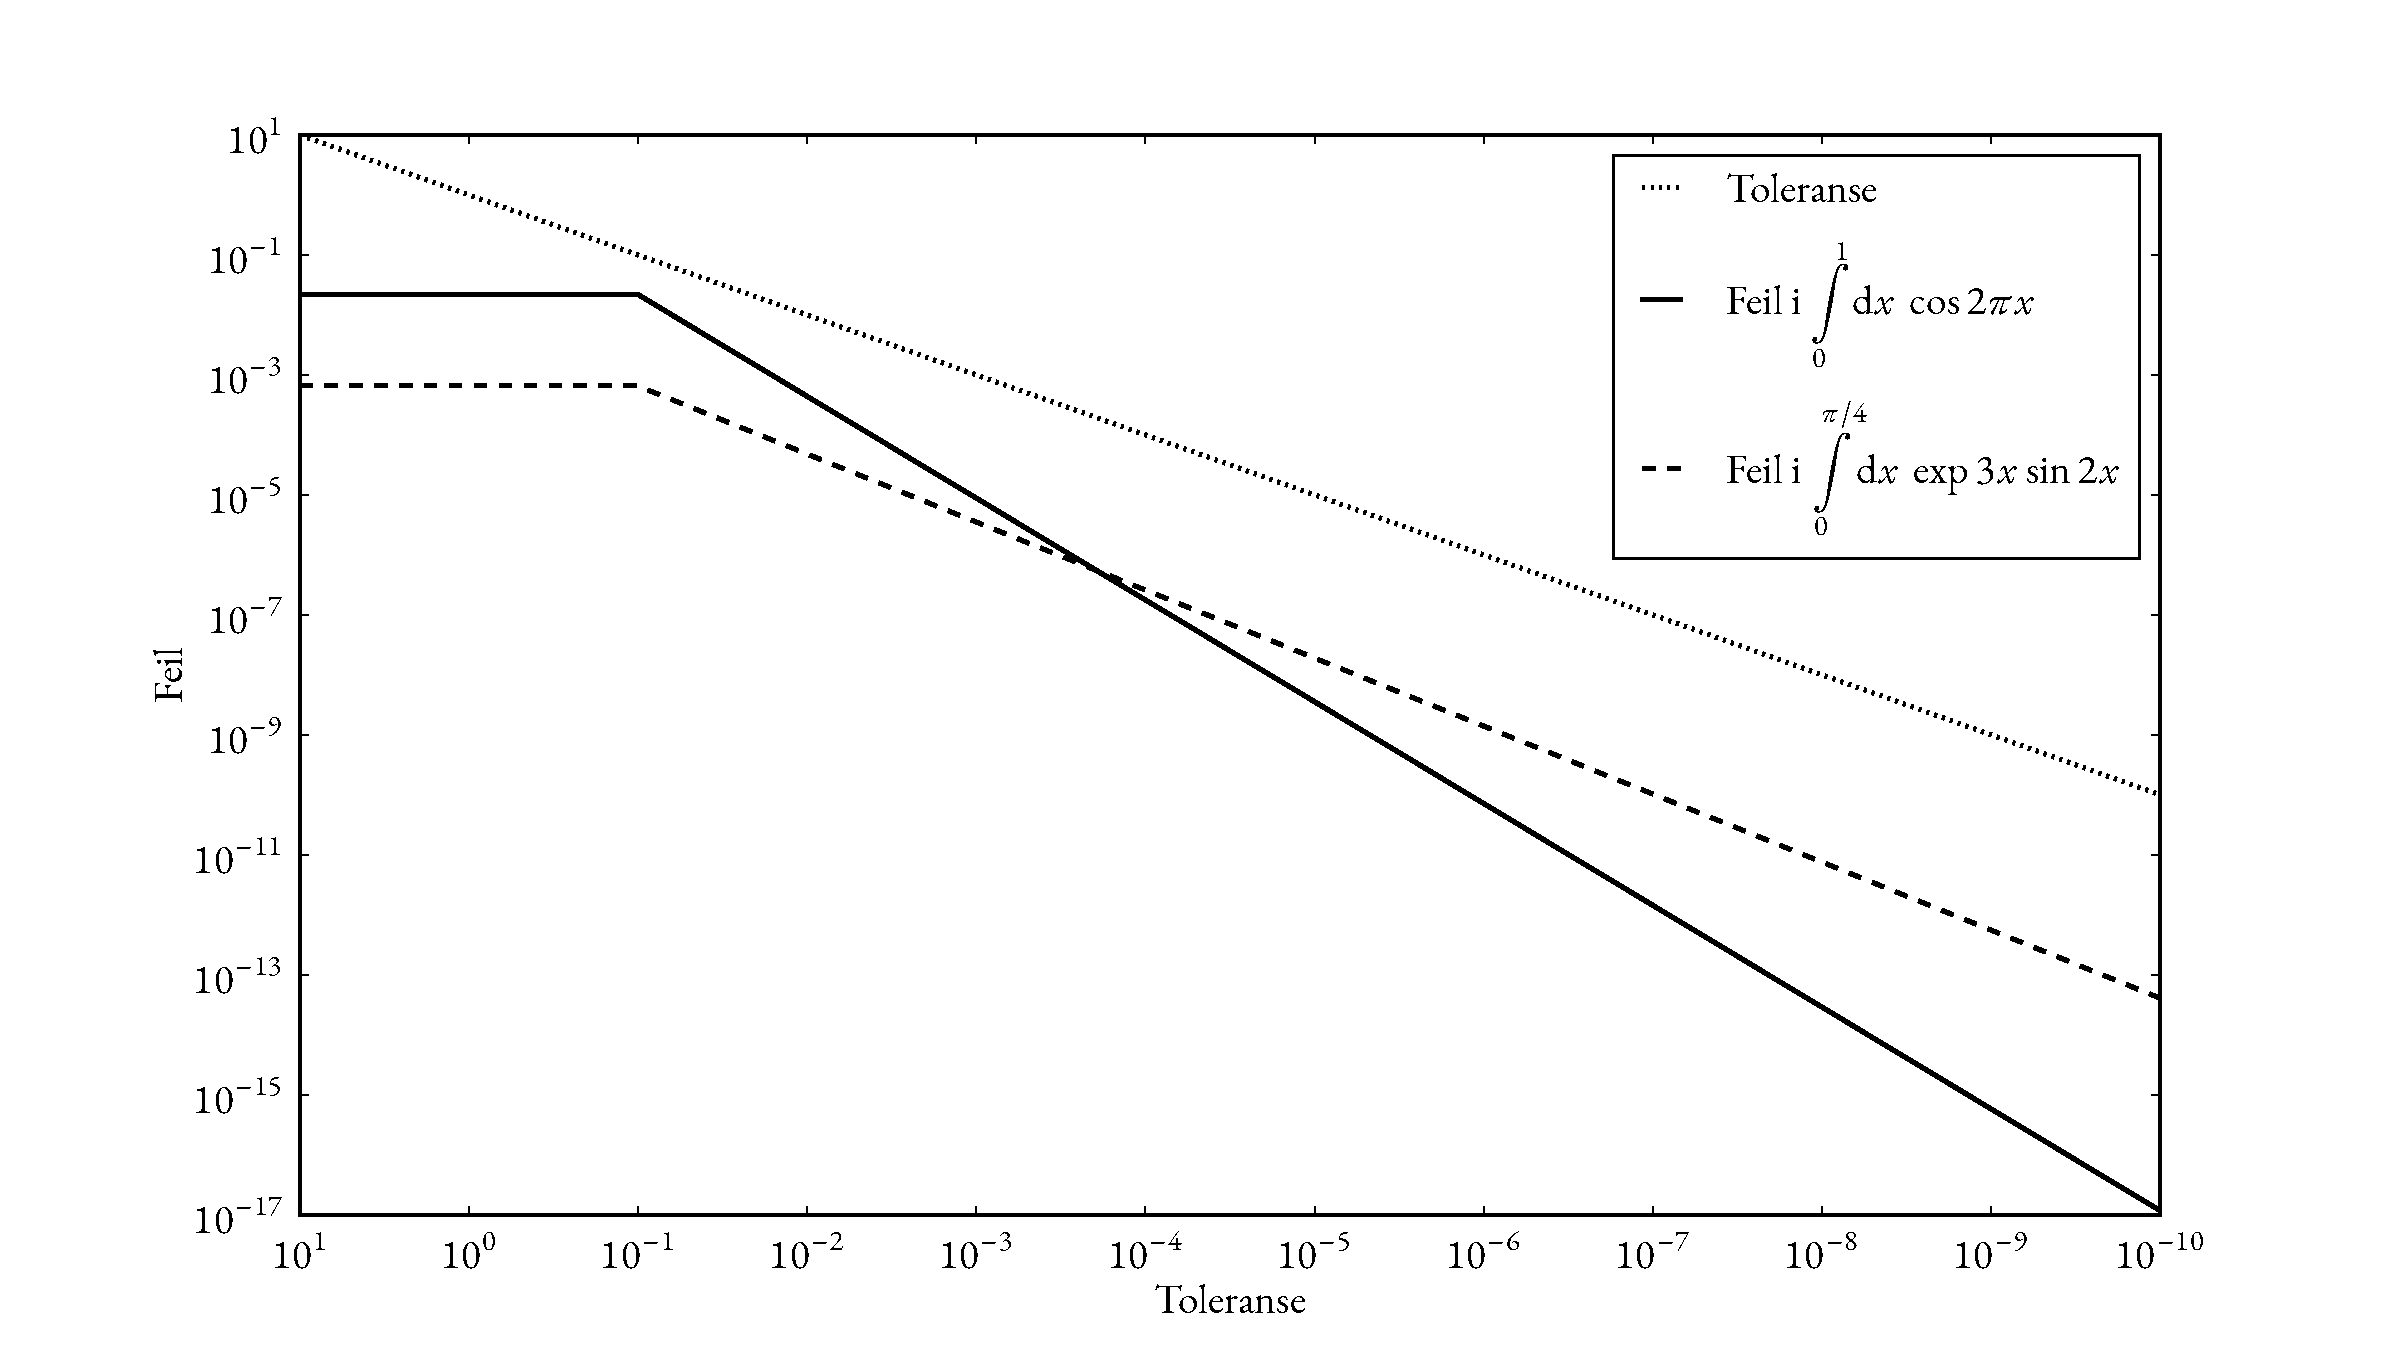
\includegraphics[width=\columnwidth]{simp_err}
        \caption{Feil i adaptiv Simpson-kvadratur.
        Ein ser at feilen er grensa ovanfrå av toleransen.}
        \label{fig:simp_err}
    \end{figure}


    \subsection{Romberg-kvadratur}
    Romberg-algoritma (\A{a_rom}) organiserer (i prinsippet) dei utrekna verdiane
    i ei nedre-triangulær matrise, der kvar {\em kolonne} er estimat av integralet
    med aukande presisjon (kortare steglengde) nedover langs kolonna.
    Trikset til Romberg er at ein -- ved hjelp av to estimat av ein gitt orden,
    med forskjellige steglengder $h$ og $h/t$ -- kan ein konstruere eit estimat
    av {\em høgare orden}, ved hjelp av {\em Richardson-ekstrapolering}.
    Ekstrapoleringa {\em aksellererer} konvergensen til følgja,
    som ein ser i \Fig{rom_err}.

    La $A(h)$ vere ein approksimasjon på ekvidistante nodar med steglengde $h$
    \[
        A(h) \approx I \coloneqq \int\limits_a^b \D{x} f(x)
    \]
    slik at $A(h) - I = \mathscr O(h^{n})$, der restfunksjonen er eit polynom i $h$.
    I tilfelle for Rombergs metode er denne gitt ved Euler-Maclaurin-ekspansjonen.
    Generelt, ved å bruke tilnærmingar med to forskjellige steglengder,
    $A(h)$ og $A(h/t)$, har vi
    \begin{align*}
        \begin{split}
            A(h/t) - A(h) =& \left(I + k\left(\frac h t\right)^n + \mathscr O\left(h^{n+1}\right)\right)\\
            -& \left(I + kh^n + \mathscr O\left(h^{n+1}\right)\right) \\
        \end{split}
    \end{align*}
    her har vi skrive ut det første leddet i rest-funksjonen;
    målet er å bli kvitt $h^n$-leddet.
    Dette oppnår vi dersom vi gongar $A(h/t)$ med $t^n$:
    \begin{align*}
        \begin{split}
            t^nA(h/t) - A(h) = t^nI - I + \mathscr O \left(h^{n+1}\right)
        \end{split}
    \end{align*}
    Her har vi innlemma $t^n$ i det asymptotiske leddet.
    Del med $t^n - 1$ og trekk $I$ frå begge sider:
    \begin{equation}
        \frac{t^nA(h/t) - A(h)}{t^n - 1} - I = \mathscr O \left(h^{n+1}\right)
    \end{equation}
    Altso har vi, ved å bruke {\em to} approksimasjonar med ulike steglengder,
    klart å hoste opp ein approksimasjon av {\em høgare orden}!
    Dersom vi startar med $N$ estimat v. h. a. trapesmetoden
    kan vi ekstrapolere $N$ gongar, og organisere approksimasjonane
    i ei nedretriangulær matrise.
    Organiserer vi utrekningane slik at kvar ekstrapolasjon $R(m, n)$ kun brukar
    dei to approksimasjonane $R(m-1, n)$ og $R(m-1,n-1)$ kan vi beregne
    approksimasjonane rad for rad, i staden for kolonne for kolonne.
    På denne måten oppnår vi ønska presisjon med ferrast mulig nodar
    i den opprinnelige trapesmetoden,
    og vi treng kun lagre to rader i gangen, så vi sparer minne.
    Denne metoden heiter {\em Rombergs metode},
    og nokre estimat av integral er i \Tab{rom}.

    \begin{table}[H]
        \centering
        \caption{
            Estimasjonar v. h. a. Rombergs metode
            med toleranse $\varepsilon = 10^{-10}$.
        }
        \label{tab:rom}
        \begin{tabular}{c c c}
            \toprule
            \sc Integral & \sc Estimat \\
            \midrule
            $ \displaystyle \int\limits_{x = 0}^{x = 1} \D{x} \cos 2\pi x $ &
            $ 3.30152344409 \times 10^{−17}$ \\
            %%%
            $ \displaystyle \int\limits_{x = 0}^{x = 1} \D{x} \, \sqrt[3] x $ &
            $ 0.74998846514 $ \psatan \\
            %%%
            $ \displaystyle\mathrm{erf}(1) = \frac 2 {\sqrt \pi} \int\limits_{x = 0}^{x = 1} \D{x} e^{-x^2} $ &
            $ 0.84270079294 $ \\
            \bottomrule
        \end{tabular}
    \end{table}

    Det ser ikkje ut til at toleransen $\varepsilon$ er ei øvre skranke for
    feilen i Rombergs metode. Feilen i (\satan) er om lag
    ${\delta = 1.15 \times 10^{-5}}$,
    som er større enn $\varepsilon = 10^{-10}$.
    For det same integralet, med den same toleransen,
    gjer den adaptive kvadraturmetoden svaret $0.75$,
    som er eksakt, men tar om lag ti gongar so lang tid å kjøre.

    \begin{figure}[H]
        \centering
        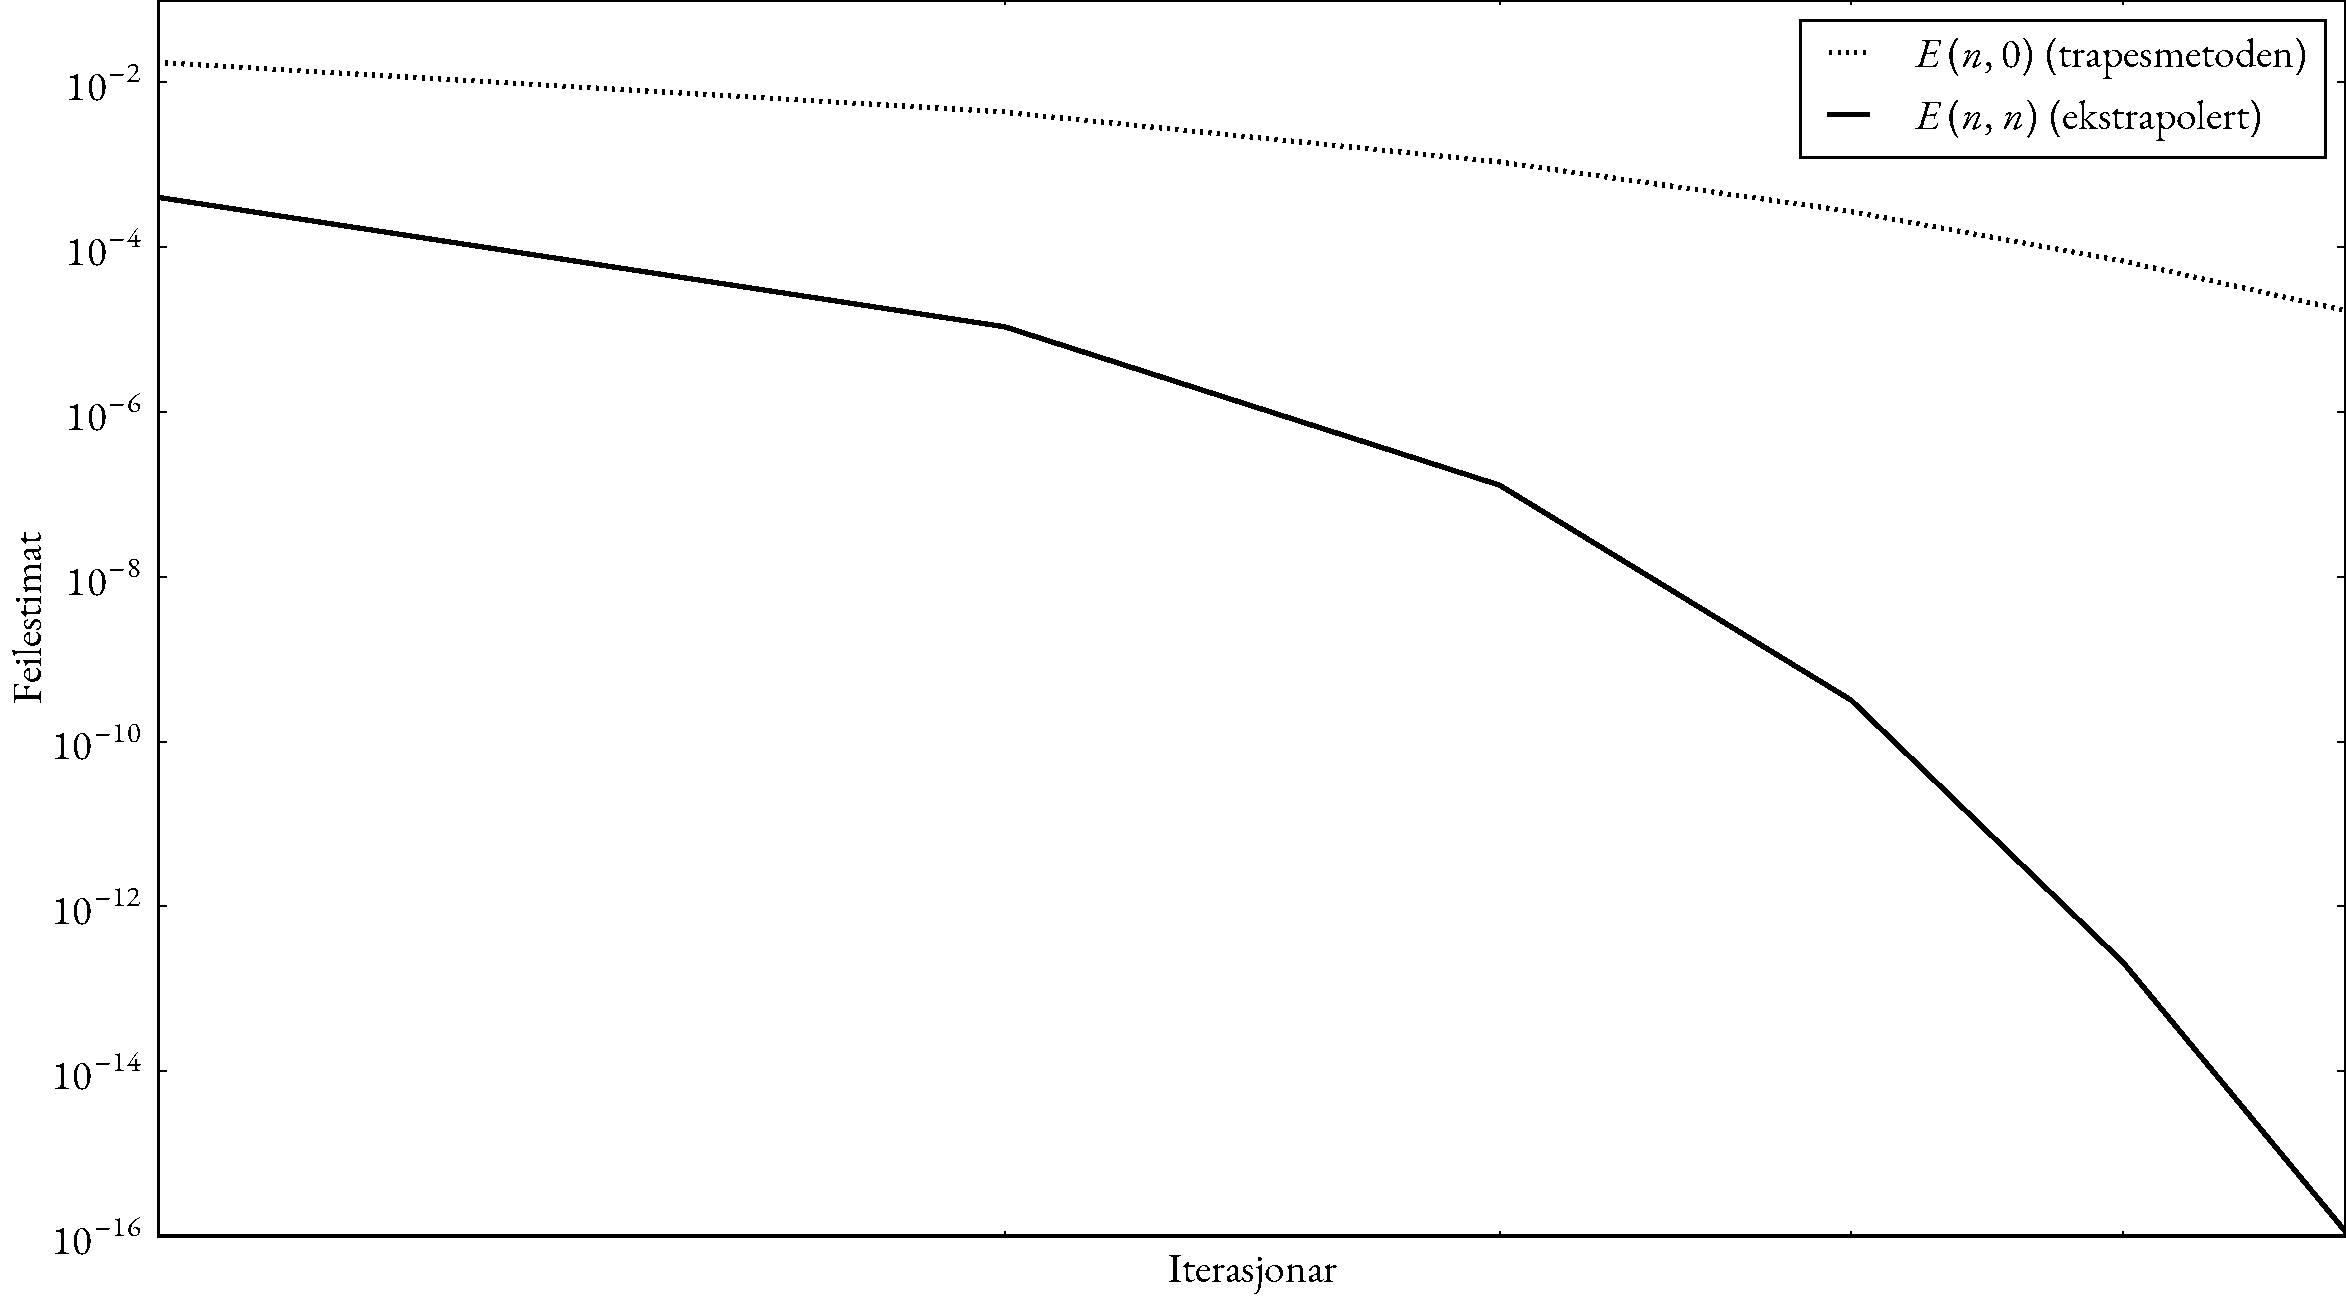
\includegraphics[width=\columnwidth]{rom_err}
        \caption{
            Feil i Rombergs metode.
            Det er tydeleg at elementa langs diagonalen kovergerer
            raskt samanlikna med elementa i første kolonne.
            Den akselererte følgja når presisjonen etter berre $6$ iterasjonar.
        }
        \label{fig:rom_err}
    \end{figure}

    \section{Simulasjon av fri, stiv lekam}
    Vi ønsker å simulere ein {\em fri, stiv lekam},
    med andre ord ein lekam som ikkje lar seg deformere,
    som roterer fritt i rommet frå ein gitt start-tilstand.

    Fri rotasjon betyr at netto påført dreiemoment er null.
    At lekamen ikkje lar seg deformere medfører at
    treighetsmomentet er konstant. (massen ``flyttar seg ikkje'' relativt
    til rotasjons-aksen)
    Dette betyr at normen til dreieimpulsen er bevart (den er fri til å endre retning),
    og rotasjonsenergien $E = \frac 1 2 T\vec \upomega^2$ er bevart. \cite{lien}

    \subsection{Definisjon av problemet}
    Differensiallikninga
    \cite{lien}
    \begin{equation}
        \Mat T \DD{t}{\vec \upomega} + \vec \upomega \times \Mat T\vec \upomega = \vec M
        \label{_euler}
    \end{equation}
    skildrar rotasjonen til eit stivt legeme.
    Her er $\vec M$ påført dreiemoment,
    $\Mat T$ treighetsmoment, og $\vec \upomega$ vinkelfart.
    Per antagelse er $\vec M = 0$. Innfør
    $\vec m = \Mat T \vec \upomega$,
    som er eit produkt av eit moment, $\Mat T$,
    og ein fart, $\vec \upomega$. Altso er $\vec m$ ein form for {\em impuls}
    -- nemleg {\em dreieimpulsen}. Vi har
    \begin{equation}\label{dreieimpuls}
        \DD{t}{\vec m} = \Mat T \DD{t}{\upomega} \quad\text{og} \quad
        \vec \upomega = \Mat T^{-1} \vec m \text.
    \end{equation}
    I \eqref{_euler},
    trekk frå $\DD*{t}{\vec m}$ på begge sider,
    og snu kryss-produktet for å få like forteikn.
    Samtidig innfører vi notasjonen $\dot f$
    for tids-deriverte.
    \begin{equation}
        \dot \vec m = \vec m \times \Mat T^{-1} \vec m
        \label{euler}
        \tag{\ref{_euler}*}
    \end{equation}
    Bevaringslovene nevnt til å byrje med, saman med \eqref{dreieimpuls}, gir
    \begin{align}
        \label{sph}
        \gamma &= \Norm{\vec m}^2 = \vec m(t) \cdot \vec m(t) \\
        \label{ell}
        E &= \frac{1}{2} \vec m(t) \cdot \Mat T^{-1} \vec m(t)
    \end{align}
    Der \eqref{sph} er ei sfære med radius  $\Norm{\vec m}$,
    og \eqref{ell} er ei ellipse.
    Sidan både $\gamma$ og $E$ er konstantar er løysingane $\vec m$ begrensa
    til å sitje på skjæringa mellom flatene.

    Anta $\Mat T = \Diag(\Mat I_1, \Mat I_2, \Mat I_3)$.
    Ettersom $\Mat T$ er diagonal er
    $\Mat T^{-1} = \Diag(1/\Mat I_1, 1/\Mat I_2, 1/\Mat I_3)$.
    Skriv $\vec m = (x \; y \; z)$, og skriv ut \eqref{euler}
    på komponentform:
    \begin{align*}
        \underset{\dot \vec m}{\begin{pmatrix}
            \dot x(t) \\ \dot y(t) \\ \dot z(t)
        \end{pmatrix}}
        =
        \underset{\vec m}{\begin{pmatrix}
            x(t) \\ y(t) \\ z(t)
        \end{pmatrix}}
        \times
        \left[
            \underset{\Mat T^{-1}}{\begin{pmatrix}
            1/\Mat I_1 &0&0 \\ 0& 1/\Mat I_2 &0 \\ 0&0& 1/\Mat I_3
        \end{pmatrix}}
        \underset{\vec m}{\begin{pmatrix}
            x(t) \\ y(t) \\ z(t)
    \end{pmatrix}}
    \right]
    \end{align*}
    Rekn ut kryssproduktet:
    \begin{align}
        \label{euler_komp}
        \underset{\dot \vec m}{\begin{pmatrix}
            \dot x(t) \\ \dot y(t) \\ \dot z(t)
        \end{pmatrix}}
        =
        \underset{f(t, \vec m)}{\begin{pmatrix}
            A y(t) z(t) \\ B x(t) z(t) \\ C  x(t) y(t)
        \end{pmatrix}}
    \end{align}
    der $A$, $B$ og $C$ er konstantar
    \begin{align*}
        A = 1/I_3 - 1/I_2 \\
        B = 1/I_1 - 1/I_3 \\
        C = 1/I_2 - 1/I_1
    \end{align*}

    \subsection{Implisitt Runge-Kutta midtpunkt-metode}
    Vi ønsker å løyse differensiallikningar av sorten
    \[
        \dot y = f(t, y)
    \]
    numerisk, ved hjelp av Runge-Kutta metoden
    \begin{equation}
        y_{n + 1} = y_n + h f\left( t_n + \frac{h}{2}, \frac{1}{2}(y_n + y_{n + 1})\right) \text,
        \label{mpm}
    \end{equation}
    kalt {\em implisitt midtpunktmetode}, fordi $y_{n+1}$ avheng
    av eit estimat for $y_{n+1/2}$ (derav implisitt)
    for å estimere tangenten i midpunktet mellom $t_n$ og $t_{n+1}$.
    Substituer
    \[
        u = \frac 1 2 (y_n + y_{n + 1}) \implies y_{n+1} = 2u - y_n
    \]
    for å forenkle notasjonen litt.
    Dette gir likningssystemet
    \[
        2u - y_n = y_n + h f\left( t + h/2, u \right) \\
    \]
    som vi kan skrive
    \begin{equation}
        u = y_n + \frac h 2 f\left( t+h/2, u \right)
    \end{equation}
    og dette må løysast med omsyn til $u$ for kvart tidssteg.
    Systemet vi er interresert i har tre variablar; $x$, $y$ og $z$.
    Med $\vec u = (x \, y \, z)$ kan vi definere
    \begin{equation}
        \vec F(\vec u) = \vec u_n + f(t_n + h/2, \vec u) - \vec u
    \end{equation}
    der $\vec u_n$ er førre iterasjon,
    og søke etter nullpunkt ved hjelp av ein kjend
    løysar for ulineære likningssystem, til dømes Newtons metode.
    (som er kjend frå tidlegare øvingar, men eg gjentar det
    mest grunnleggande for kompletthets skyld)

    Gitt Jacobian-matrisa til $\vec F$, $\mathscr J_\vec F$,
    kan vi bruke den iterative prosessen
    \[
        \vec u \longleftarrow \vec u - \mathscr J^{-1}_\vec F \vec F(\vec u)
    \]
    med $\vec u = \vec u_n$ som startverdi.
    Iterasjonen er slutt når antal iterasjonar har nådd ei øvre grense,
    eller når $\Norm{\vec F(\vec u)} < \varepsilon$,
    for ein gitt toleranse $\varepsilon$.
    Med $y_{n+1/2} = \vec u$ reknar vi ut $y_{n+1}$:
    \begin{equation}
        \label{impl_RK}
        y_{n+1} = y_n + h f\left(t + h/2, y_{n+1/2}\right)
    \end{equation}
    og dette fullfører \'ein iterasjon av Runge-Kutta-metoden.



    \subsection{Implementasjon av RK-metoden}
    Vi brukar eit symbolsk verktøy for å rekne ut \eqref{impl_RK}
    i forkant, til dømes {\tt sympy}.
    Den eine haka ved denne implementasjonen er at differensiallikninga vi
    vil løyse må vere definert berre ved hjelp av
    funksjonar som er kompatible med {\tt sympy},
    men det er enklare å ha eit eksplisitt uttrykk for
    Jacobian-matrisa ved kvart tidssteg.

    Det er enklare å
    behandle uttrykk der dimensjonen er kjend.
    {\tt sympy} {\em har} funksjonalitet for å lage
    vektorar med symbol, så det er (i prinsippet) mogleg
    å implementere metoden for $N$ dimensjonar,
    men element i desse vektorane får obskure navn som gjer feilsøking til eit mareritt.
    Implementasjonen (\A{a_rk}) er derfor begrensa til tre dimensjonar.

    \subsection{Modifisert Eulers metode}
    Vi implementerer \`og den eksplisitte RK-metoden (\A{a_euler})
    \begin{align*}
        y_{n+1/2} &= y_n + \frac h 2 f\left(t_n, y_n\right) \\
        y_{n+1} &= y_{n+1/2} + h f\left(t_n + 1/2, y_{n+1/2}\right) \\
    \end{align*}
    for å samanlikne den implisitte metoden med ein eksplisitt metode.
    Metoden treng ingen forklaring, sidan den er eksplisitt.

    \subsection{Numerisk Løysing av Likninga}
    I \Lst{lst:solver} vert bruk av løysarane demonstrert.

    \noindent\begin{minipage}{\linewidth}
    \begin{python}[caption={Bruk av RK-løysarane},label=lst:solver]
def f(t, m):
    x, y, z = m
    return [ (1/I3 - 1/I2) * y * z ,
             (1/I1 - 1/I3) * x * z ,
             (1/I2 - 1/I1) * x * y ]

t = np.linspace(0, 150, 150)

y0 = np.array([2, 3, 4], dtype=float)
y0 *= 1/linalg.norm(y0)

x, y, z = RK(f, y0 = y0, t = t)
    \end{python}
    \end{minipage}


    \subsection{Kvadratisk konvergens}
    Vi brukar ei svært nøyaktig algoritme frå \verb|sympy|,
    med svært kort steglengde,
    for å estimere $\vec m(t = 1)$ so nøyaktig som mogleg.
    Dersom vi antar at denne verdien er om lag eksakt,
    samanlikna med verdiane vi oppnår med våre metodar med
    relativt lange steglengder kan vi undersøkje korleis
    feilen oppførerseg når steglengda minkar.
    Feilen kan ein sjå i \Fig{kvad_err}, med steglengda som abscisse.

    Ved sidan er der teikna ei linje $y = h^2$.
    I \verb|loglog|-plottet har denne stigningstal $m = 2$.
    ($\log x^2 = 2 \log x$)
    Det er heilt klart at begge metodana har same stigningstal som linja,
    altso er begge kvadratisk konvergente i $h$,
    RK med litt lågare konstantfaktor enn Euler.
    \begin{figure}[H]
        \centering
        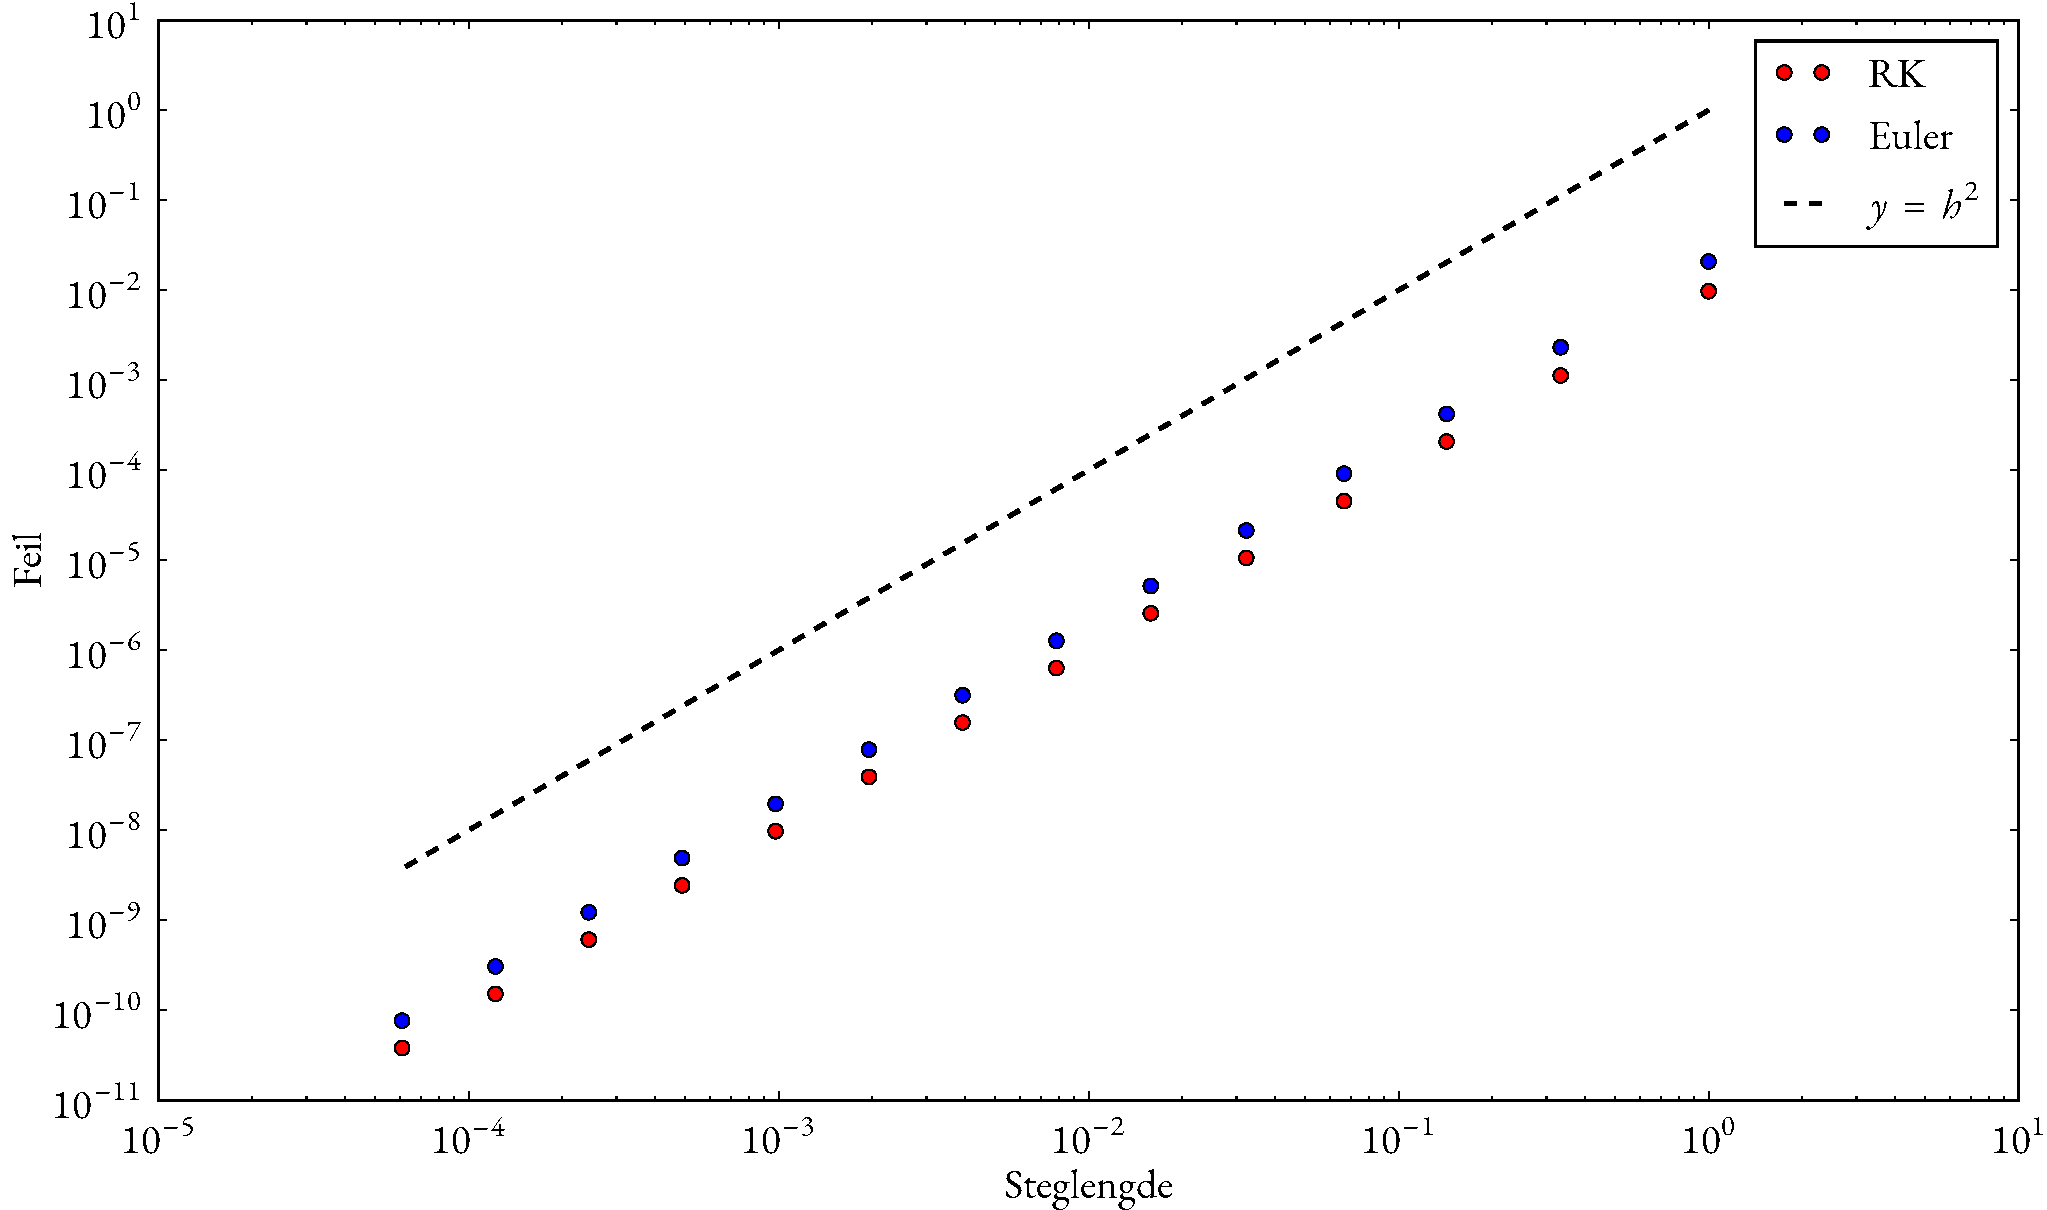
\includegraphics[width=\columnwidth]{kvad_err}
        \caption{
            Feilen i begge metodane er tydeleg kvadratiske.
        }
        \label{fig:kvad_err}
    \end{figure}
    \noindent Merk at dette tidsrommet er svært kort.
    Vi er \`og interreserte i å undersøkje kvar som skjer over
    lange tidsrom.

\end{multicols}
\noindent\begin{minipage}[!b]{\textwidth}
    \nablarule
    \begin{figure}[H]
        \centering
        \begin{subfigure}{.4\textwidth}
        \centering
        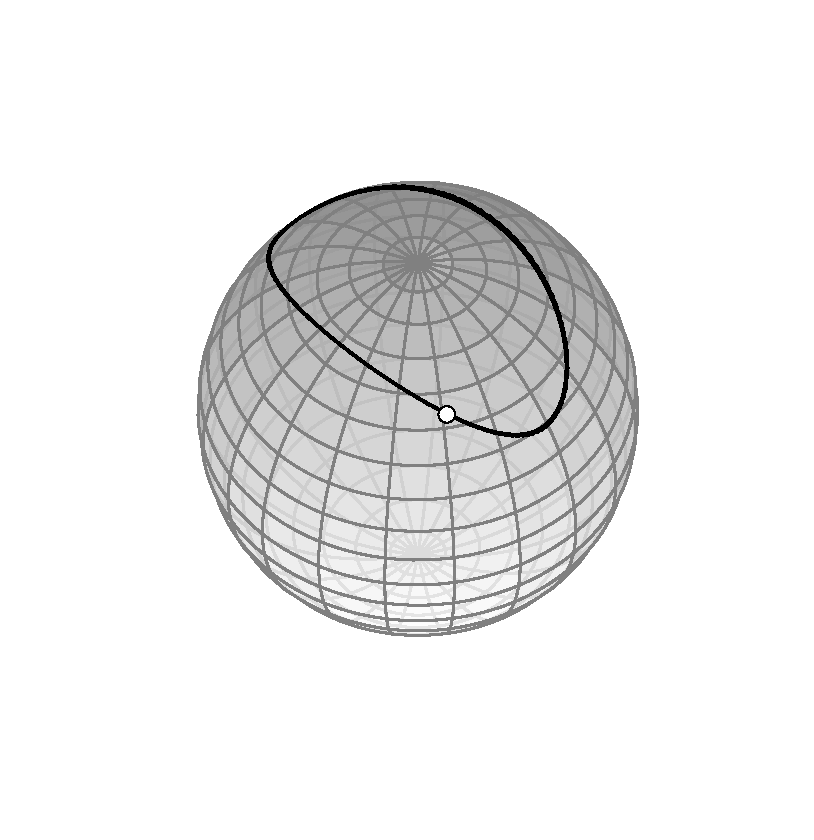
\includegraphics[width=\linewidth]{rk}
        \caption{
            Løysing v. h. a. implisitt midtpunkt-metode.
            Løysinga er presis, sjølv etter svært lang tid.
        }
        \label{fig:rk}
    \end{subfigure} \hspace{.05\textwidth}
        \begin{subfigure}{.4\textwidth}
        \centering
        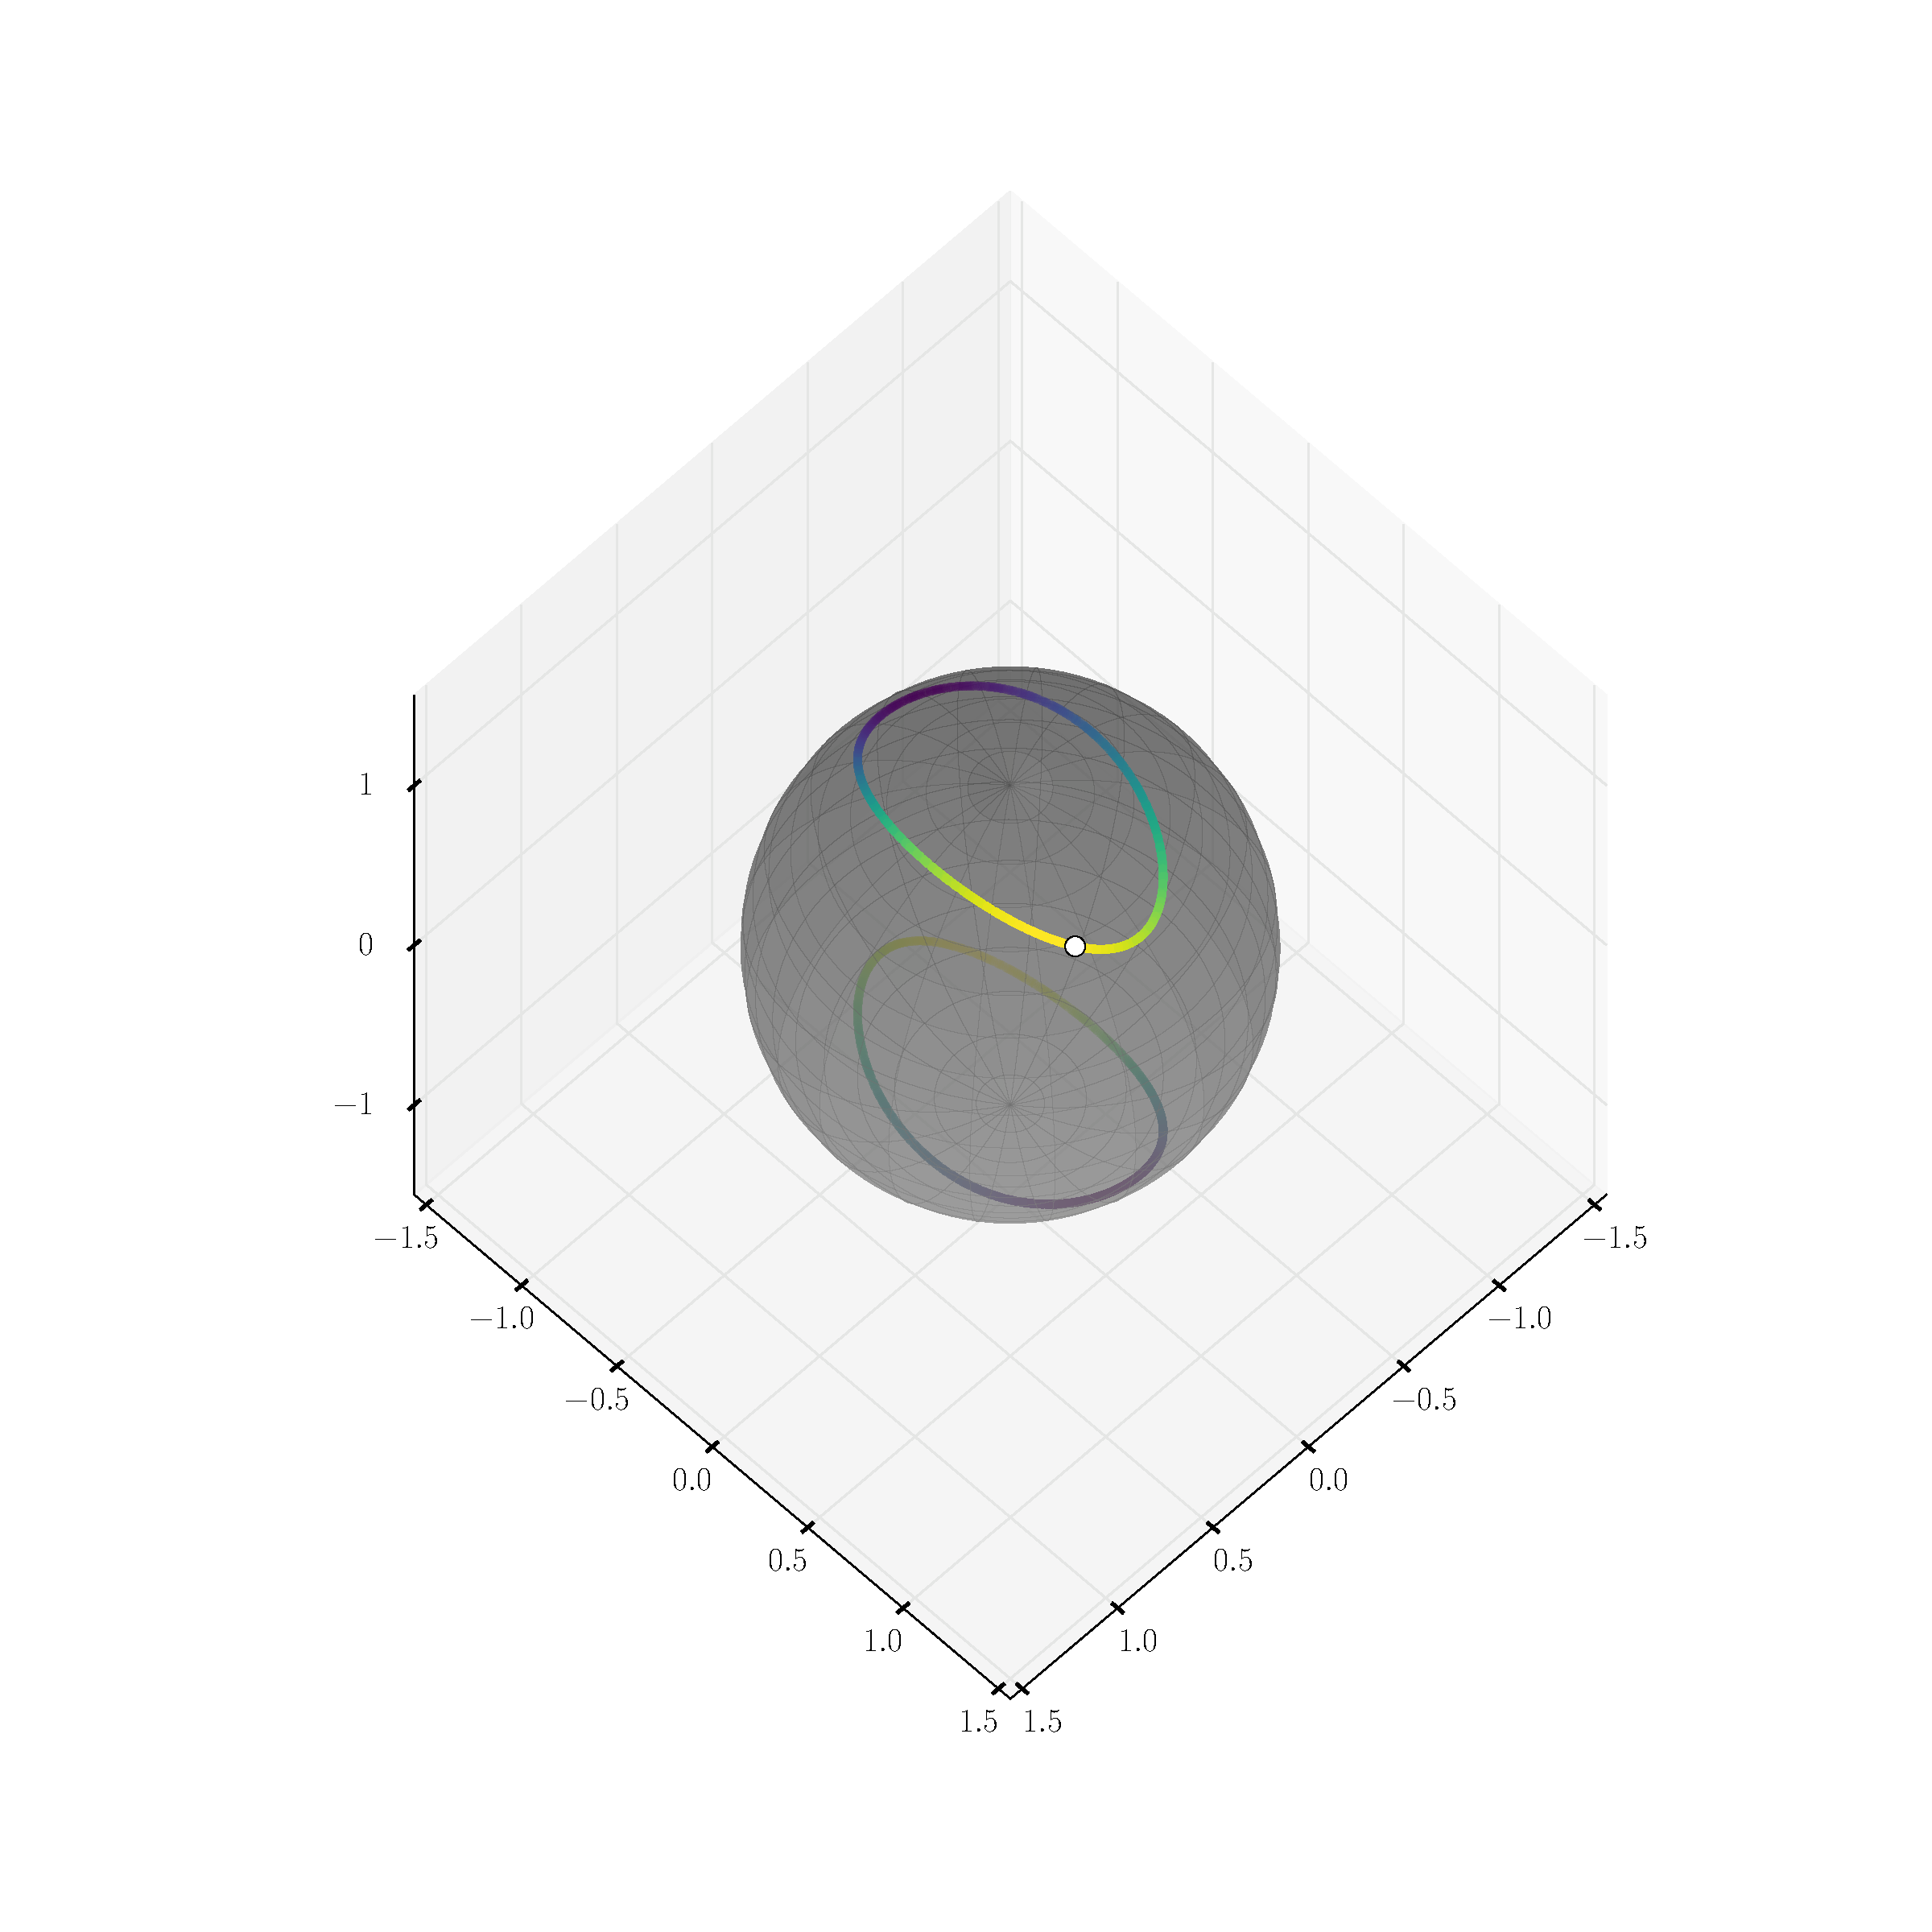
\includegraphics[width=\linewidth]{euler}
        \caption{
            Løysing v. h. a. eksplisitt modifisert Eulers metode.
            Løysinga vert ubrukeleg nesten med ein gang.
        }
        \label{fig:euler}
        \end{subfigure}
        \caption {
            Løysingar av \eqref{euler} med initialverdiar
            $\Mat T = \Diag(1, 2, 5)$ og $\vec m_0 = (2 \; 3 \; 4)$.
            Tidsrommet er $t = 150$, med $N = 150$ steg.
            Initialverdien $\vec m_0$ er markert.
            Løysingane er plotta på ei sfære $\gamma = \Norm{\vec m_0}^2$.
        }
        \label{fig:loysingar}
    \end{figure}
    \hrule
\end{minipage}
\begin{multicols*}{2}

    \subsection{Lange tidsrom}

    \noindent Løysingane produsert av løysarane er plotta i
    \Fig{rk} (implisitt RK) og \Fig{euler} (eksplisitt modifisert Euler).
    Det er tydeleg at den implisitte metoden produserer
    langt meir presise løysingar til dette initialverdiproblemet
    over lang tid:
    Den eksplisitte løysinga forl\'et sfæra nesten umiddelbart,
    og feilen veks raskt til å verte urimeleg stor.



\printbibliography

\end{multicols*}

\newpage
\newgeometry{
    left=3.5cm,
    right=3.5cm
}
\fancyhead[C]{\sc Appendix}
\fancyhfoffset[O]{0pt}

\begin{appendices}

    \section{Simpson-kvadratur} \label{a_simp}
    \noindent\begin{minipage}{\linewidth}
    \begin{python}[caption={Adaptiv Simpson-kvadratur}]
def S(f, a, b):
    return (f(a) + 4 * f((a + b) / 2) + f(b))  \
         * (b - a) / 6

def asm_quad(f, a, b, tol=1e-5):
    I0 = S(f, a, b)
    c = (a + b) / 2

    I = S(f, a, c) + S(f, c, b)
    err = abs(I - I0) / 15

    if err < tol:
        return I + (I - I0) / 15
    else:
        return asm_quad(f, a, c, tol=tol/2)  \
             + asm_quad(f, c, b, tol=tol/2)
    \end{python}
    \end{minipage}


    \section{Romberg-kvadratur} \label{a_rom}
    \noindent\begin{minipage}{\linewidth}
    \begin{python}[caption={Romberg-kvadratur}]
def romberg(f, a, b, MAX_ITER=100, tol=1e-5):
    R = np.zeros((2, MAX_ITER))
    Rp, Rn = 0, 1

    h = b - a
    R[Rp, 0] = 0.5 * h * (f(a) + f(b))

    for n in range(1, MAX_ITER):
        h = h * 0.5
        L = np.linspace(a + h, b - h, 1 << n - 1)
        R[Rn, 0] = R[Rp, 0]/2 + np.sum(f(L))*h

        for k in range(1, n + 1):
            E = (R[Rn, k - 1] - R[Rp, k - 1])  \
              / ((1 << 2 * k) - 1)
            R[Rn, k] = R[Rn, k - 1] + E

        Rp, Rn = Rn, Rp

        if abs(E) < tol: break

    return R[Rp, n]
    \end{python}
    \end{minipage}


    \section{Implisitt Runge-Kutta} \label{a_rk}
    {\tt sympy}-koden for likningssystemet er ikkje spesielt vanskelig,
    men den er lang og stygg, så eg har klipt den ut.
    Algoritma kan finnast i jupyter-notebook: {\tt rk3d.pynb},
    og der er sjølvsagt {\tt sympy}-koden inkludert.

    \noindent\begin{minipage}{\linewidth}
    \begin{python}[caption={Implisitt Runge-Kutta midtpunktmetode.}]
def RK(f, y0, t):

    # (Sympy-junk removed here...)

    y = np.empty((len(t), 3))
    y[0] = y0

    for n in range(len(t) - 1):
        h = t[n + 1] - t[n]

        u = newton(
            lambda u:  F(u, y[n], t[n] + h/2, h),
            lambda u: Ji(u, y[n], t[n] + h/2, h),
            y[n]
        )

        m = np.array(f(t[n] + h/2, u), dtype=float)

        y[n + 1] = y[n] + h * m

    return y.T
    \end{python}
    \end{minipage}
    I metoden inngår Newtons metode;
    denne har vi implementert i ei tidlegare øving,
    men legg den ved for kompletthets skuld:

    \noindent\begin{minipage}{\linewidth}
    \begin{python}[caption={Newtons metode frå tidlegare øving.}]
def newton(F, Ji, u0, tol=1e-10, maxiter=10):
    u = u0
    for _ in range(maxiter):
        u = u - Ji(u).dot(F(u))

        if linalg.norm(F(u)) < tol:
            break

    return u
    \end{python}
    \end{minipage}

    \section{Modifisert Euler} \label{a_euler}
    \noindent\begin{minipage}{\linewidth}
        \begin{python}[caption={Modifisert Eulers metode (eksplisitt)}]
def euler(f, y0, t):
    y = np.empty((len(t), 3))
    y[0] = y0

    for n in range(len(t) - 1):
        h = t[n + 1] - t[n]

        u = y[n] + np.array(f(t[n], y[n])) * h / 2
        m = np.array(f(t[n] + h/2, u), dtype=float)
        y[n + 1] = y[n] + h * m

    return y.T
    \end{python}
    \end{minipage}

\end{appendices}
\end{document}
